\documentclass{article}
\usepackage{graphicx} % Required for inserting images
\usepackage{minted}

\title{Numerical Methods for ODEs}
\author{Alex Zhou}
\date{April 2019}

\begin{document}

\maketitle

\section{Introduction}

We are concerned with using numerical step-by-step integration to solve simple ordinary differential equations. Given a function \(f\), an interval \([a,b]\) and initial condition \(y_0\), consider the initial value problem
\[ \frac{dy}{dx} = f(x,y),  \]
subject to \(y(a) = y_0\). We want to find a numerical approximation to the unknown function \(y\) for values in \(x \in [a,b]\). Let the exact solution be denoted as \(y = y_e(x)\). We are interested in the following numerical methods:
\begin{enumerate}
    \item (Forward) Euler method, which is a single-step method
    \[ Y_{n+1} = Y_n + hf(x_n, Y_n), \]
    where \(y_n\) denotes the numerical solution at the \(n\)th step with length \(h\), \(x_n = x_0 + nh\).
    \item Adams-Bashforth method, a two-step method
    \[ Y_{n+1} = Y_n + h\left(\frac{3}{2}f(x_n, Y_n) - \frac{1}{2}f(x_{n-1}, Y_{n-1})\right), \]
    where the first step must be taken by a single-step method.
    \item Runge-Kutta method, more specifically the fourth-order variant
    \[ Y_{n+1} = Y_n + \frac{1}{6}h(k_1 + 2k_2 + 2k_3 + k_4), \]
    where
    \begin{eqnarray*}
        k_1 &=& f(x_n, Y_n) \\
        k_2 &=& f(x_n + \textstyle\frac{1}{2}h, Y_n + \frac{1}{2}hk_1) \\
        k_3 &=& f(x_n + \textstyle\frac{1}{2}h, Y_n + \frac{1}{2}hk_2) \\
        k_4 &=& f(x_n + h, Y_n + hk_3),
    \end{eqnarray*}
    which is also a two-step method.
\end{enumerate}
In particular, we shall analyse the stability and accuracy of the three methods, as well as the trade-off between the two in applications. We define the global error after the \(n\)th step to be
\[ E_n = Y_n - y_e(x_n), \]
and the local error of the \(n\)-nth step is,
\[ e_n = Y_n - \tilde{y}_e(x_n), \]
where \(\tilde{y}_e(x)\) is the exact solution to the differential equation with initial condition \(y = Y_{n-1}\) at \(x = x_{n-1}\). A numerical method is said to be of order \(p\) or \(p\)th order accurate if the local error satisfies \(e_n = O(h^{p+1})\) as \(h \to 0\). The Euler method can be shown to be of first-order, Adams-Bashforth is second-order and our particular variant of the Runge-Kutta method is of fourth-order.

Accuracy is a statement about the limiting behaviour as \(h \to 0\), but it says nothing about behaviour at finite \(h\). The method could be unstable, where we have divergence or unboundedness of the global error. The initial value problem that we will analyse is
\[f(x, y) = -8y + 6e^{-2x}, \]
with initial condition \(y(0) = 0\). By solving the inhomogeneous linear equation analytically, (for example by separation of variables, or an exponential ansatz), the exact solution is given by
\[ y = y_e(x) = e^{-2x} - e^{-8x} \]
for all \(x > 0\).

\section{Euler Method}
A simple implementation of the Euler method in Python is given below:

\begin{minted}[autogobble, linenos]{python}
    import math
    def euler(f, h, x_start, y_start, x_end):
        n = int((x_end - x_start) / h + 1)
        x = [x_start + i * h for i in range(n)]
        y = [y_start] * n
        for i in range(n - 1):
            y[i+1] = y[i] + h * f(x[i], y[i])
        return x, y
\end{minted}

Running this on our initial value problem of interest, starting at \(y(0) = 0\) with step-size \(h = 0.5\), then comparing with the true analytic solution, we tabulate:

\begin{verbatim}[Output]
    f = lambda x, y: -8 * y + 6 * math.exp(-2 * x)
    y_e = [math.exp(-2*i*h) - math.exp(-8*i*h) for i in range(n)]
    
    x       Y                       y_e
    0.0     0                       0.0
    0.5     3.0                     0.34956380228270817
    1.0     -7.896361676485673      0.13499982060871019
    1.5     24.09509087916686       0.049780924155510616
    2.0     -72.135911432397        0.018315526353559458
    2.5     216.4626812138572       0.006737944937931844
    3.0     -649.3678298005743      0.002478752138915013
\end{verbatim}

Notice that the error oscillates wildly and the magnitude can be seen to grow exponentially. First, we compute the analytic solution of the Euler method difference equation,
\[  Y_{n+1} = Y_n + hf(x_n, Y_n) = -3Y_n + 3e^n. \]
The general solution of the homogeneous part is given by \(Y^{(h)}_n = A(-3)^n\), whilst if we try an ansatz \(Y^{(p)}_n = Be^n\) for the particular solution, by substitution we obtain \(B = \frac{3e}{3e + 1}\). Taking into account the initial value \(Y_0 = 0\), we get the formula
\[ Y_n = \frac{3e}{3e + 1}(e^{-n} - (-3)^n). \]
When comparing these iterations to that of the exact solution, we see the exponential term with the positive power will dominate and lead to a divergence from the exact solution at discrete times. We can plot the logarithm of the global error against \(x_n\) to observe the growth of the global error.

\begin{figure}
    \centering
    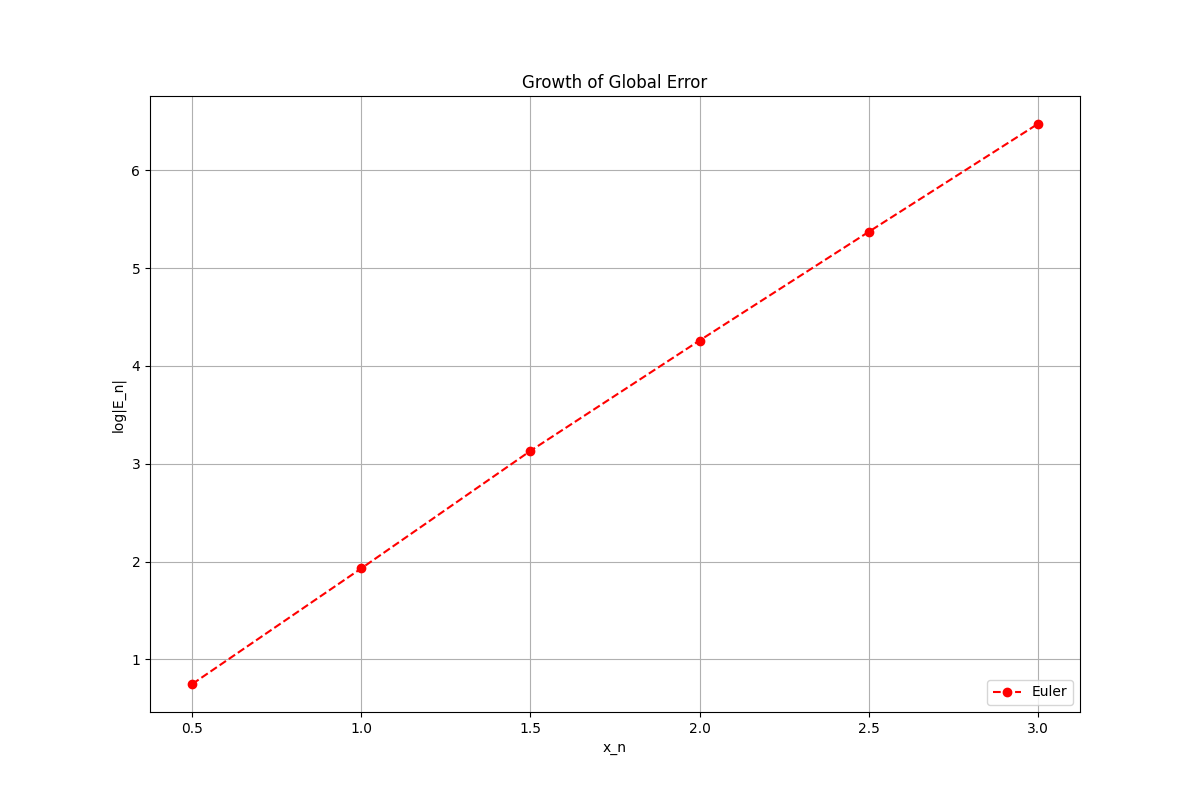
\includegraphics[width=1.0\textwidth]{images/global_error.png}
    \caption{Exponential growth of the global error for large \(h\).}
\end{figure}


We can observe that the growth is proportional to \(e^{\gamma x}\), where \(\gamma\) lies between \(2\) and \(3\). More specifically, this happens because a large \(h\) value leads to the base of the exponent to be greater than \(1\). Instead, taking a smaller \(h = 0.1\) gives us the following table:
\begin{verbatim}[Output]
    x       Y                       y_e
    0.0     0 0.0
    0.05    0.30000000000000004     0.2345173720003202
    0.1     0.4514512254107879      0.36940178896076026
    0.15    0.5164899611698673      0.43962400876951585
    0.2     0.5321394429064358      0.46842352804098397
    ...
    2.8     0.0036391828863374057   0.003697863529499291
    2.85    0.0032928688467473233   0.0033459653321323913
    2.9     0.0029795109452897756   0.0030275546613586484
    2.95    0.00269597299078661     0.0027394447624499788
\end{verbatim}
This demonstrates stability for sufficiently small \(h\) and verfies that our methods do approximate the solution closely. Analytically, we are reducing the base of the positive power exponential term since the (negative) coefficient in the difference equation of \(Y_n\) is \(8h - 1\). For this to be less than \(1\), we require \(h < 0.25\). In fact, at the boundary of divergence to infinity and convergence \(h = 0.25\), we observe oscillatory divergence.

\section{Adams-Bashforth Method}

The following is an implementation in Python where the first step is taken using the Euler method:

\begin{minted}[autogobble, linenos]{python}
    def adams_bashforth(f, h, x_start, y_start, x_end):
        n = int((x_end - x_start) / h + 1)
        x = [round(x_start + i * h, 8) for i in range(n)]
        y = [y_start] * n
        # Euler method for first step
        y[1] = y[0] + h * f(x[0], y[0])
        for i in range(1, n - 1):
            y[i+1] = y[i] + h*( (3/2) * f(x[i], y[i]) - (1/2) * f(x[i-1], y[i-1]))
        return x, y
\end{minted}

For our initial value problem of interest, we first solve the Adams-Bashforth difference equation analytically. The recurrence is given by
\[ Y_{n+1} = Y_n + h[-12Y_n + 9((e^{-2h})^n + 4Y_{n-1} - 3(e^{-2h})^{n-1}] \]
with initial condition \(Y_0 = 0\) and first step given by the Euler method \(Y_1 = 6h\). The homogenous equation is given by \(Y^{(h)}_n = Ar_{+}^n + Br_{-}^n\), where the roots of the characteristic polynomial are
\[ r_{\pm} = \frac{1}{2}\left[(1-12h) \pm \sqrt{(12h-1)^2 + 16h}\right]. \]
Trying an ansatz of \(Y^{(p)}_n= (Ke^{-2h})^n\), we obtain
\[ K = \frac{9he^{-2h} -3h}{(e^{-2h})^2 + (12h-1)e^{-2h} - 4h}. \]
Taking into account the initial conditions, we find the values for \(A, B\)
\[ A = \frac{6h + K(r_{-} - e^{-2h})}{r_+ - r_-}, \quad B = -K - A. \]
We see that the positive root \(r_+\) is always less than \(1\) for any \(h > 0\) as \(r_+\) is decreasing in \(h\) (seen by taking the derivative with respect to \(h\) and at \(h = 0\), \(r_+ = 1\)). Therefore, instability is governed by the negative root \(r_+\). Note that \(r_-\) is greater than \(1\) which happens when \(h > 1/8\) (again, it is monotonic decreasing which is seen by taking a derivative). Then, similar as before for the Euler method, the global error oscillates and diverges to infinity. 

Taking the limit as \(h \to 0\), by L'Hopital's rule, \(K \to 1\); by computation \(r_+ \to 1\) and \(r_- \to 0\); and therefore \(A \to -1\) and \(B \to 0\). Fix \(x_n = nh\). By expanding asymptotically \(\sqrt{(12h-1)^2 + 16h} \approx 1 - 4h + O(h^2)\),
\[ r_+ = \frac{(1 - 12h) + \sqrt{(12h-1)^2 + 16h}}{2} \approx 1 - 8h + O(h^2), \]
hence \(\log(r_+) \approx-8h + O(h)\) and we finally obtain \(r_+^n \approx e^{\frac{x}{h}(-8h)} = e^{-8x}\). Altogether, we get
\[ Y_n = Ar_+^n + Br_-^n + K(e^{-2h})^n \approx -1\cdot e^{-8x} + 0 + 1\cdot e^{-2x} + O(h^2), \]
which converges to the exact solution of the ODE as \(h \to 0\) and \(n \to \infty\), as required. Changing the first step to a more accurate method such as RK4 only changes the coefficients \(A, B\). In particular, this does not change the roots of the characteristic polynomial, so the divergence of the global error still occurs at the same large values of \(h\).

\section{Runge-Kutta Method}

Below is an implementation of the fourth-order Runge-Kutta method.

\begin{minted}[autogobble, linenos]{python}
    def runge_kutta(f, h, x_start, y_start, x_end):
        n = int((x_end - x_start) / h + 1)
        x = [round(x_start + i * h, 8) for i in range(n)]
        y = [y_start] * n
        for i in range(n - 1):
            # Compute intermediate values
            k1 = f(x[i], y[i])
            k2 = f(x[i] + (h/2), y[i] + (h/2)*k1)
            k3 = f(x[i] + (h/2), y[i] + (h/2)*k2)
            k4 = f(x[i] + h, y[i] + h*k3)
            y[i+1] = y[i] + (h/6) * (k1 + 2*k2 + 2*k3 + k4)
        return x, y
\end{minted}

Taking step-size \(h = 0.8\) and initial condition \(Y_0 = 0\) on the interval \([0,2]\), we can compare our three methods to the exact solution via the following table and plot.

\begin{verbatim}[Output]
    x       Euler       AB2         RK4         Exact
    0.0     0.0         0.0         0.0         0.0
    0.08    0.48        0.48        0.32410708  0.32485136
    0.16    0.58182902  0.39274353  0.44734673  0.44811174
    0.24    0.55800998  0.48762254  0.47159378  0.47217643
    0.32    0.49789962  0.4164311   0.44960068  0.44998768
    0.4     0.43234423  0.40383899  0.40833325  0.40856676
    ...
    1.6     0.03975638  0.0409047   0.0407673   0.04075944
    1.68    0.03387816  0.0348631   0.03474052  0.0347338
    1.76    0.02886906  0.02971049  0.02960441  0.02959867
    1.84    0.02460059  0.02531974  0.02522747  0.02522257
    1.92    0.02096324  0.02157682  0.02149757  0.02149339
    2.0     0.0178637   0.01838727  0.01831909  0.01831553
\end{verbatim}

\begin{figure}
    \centering
    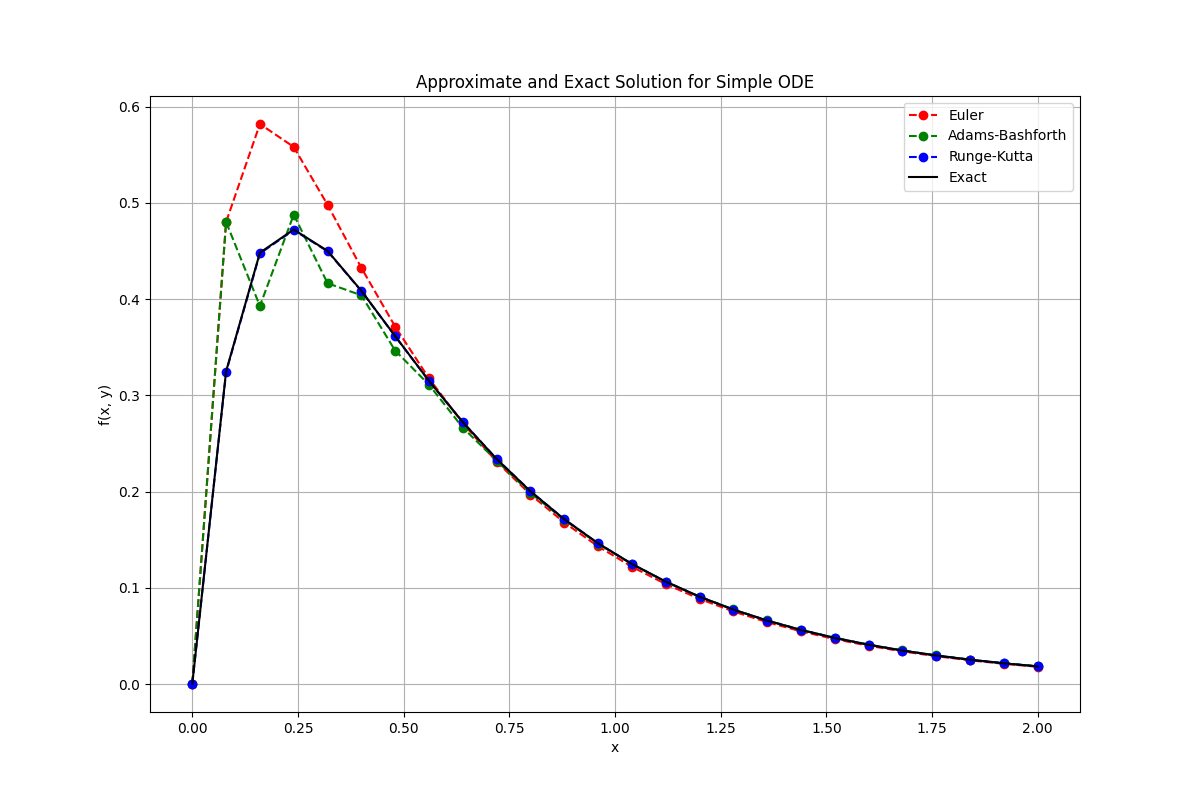
\includegraphics[width=1.0\linewidth]{images/ODE_comparison.png}
    \caption{\(y' = -8y+6e^{-2x}\).}
\end{figure}

We analyse the global error of the three methods by taking step-sizes \(h = 0.16 / n\), where \(n = 2^k\) for \(k = 0, \dots, 15\). This give us the information of the cumulative local errors up to \(x_n = 0.16\), of which there are \(1.6 / h\). We tabulate the results for the Runga-Kutta method below:

\begin{verbatim}[Output]
    h               E_n(h)
    0.16            -0.021515851003511943
    0.08            -0.0007650066799523292
    0.04            -3.6098200158984906e-05
    0.02            -1.962196212401679e-06
    0.01            -1.1439171604399334e-07
    0.005           -6.905267468937382e-09
    0.0025          -4.241488826828288e-10
    0.00125         -2.6280255749355774e-11
    0.000625        -1.6353030041216243e-12
    0.0003125       -1.0202949596305189e-13
    0.00015625      -5.828670879282072e-15
    7.8125e-05      -5.921206303050042e-10
    3.90625e-05     -2.962885492507894e-10
    1.953125e-05    -1.4833290151727851e-10
    9.765625e-06    -7.381995015265375e-11
    4.8828125e-06   -3.695443950846311e-11
\end{verbatim}

Using these results, as well as those for the other two methods, we can plot a log-log graph of the global error at \(x_n = 1.6\) over the step-size \(h\).

\begin{figure}
    \centering
    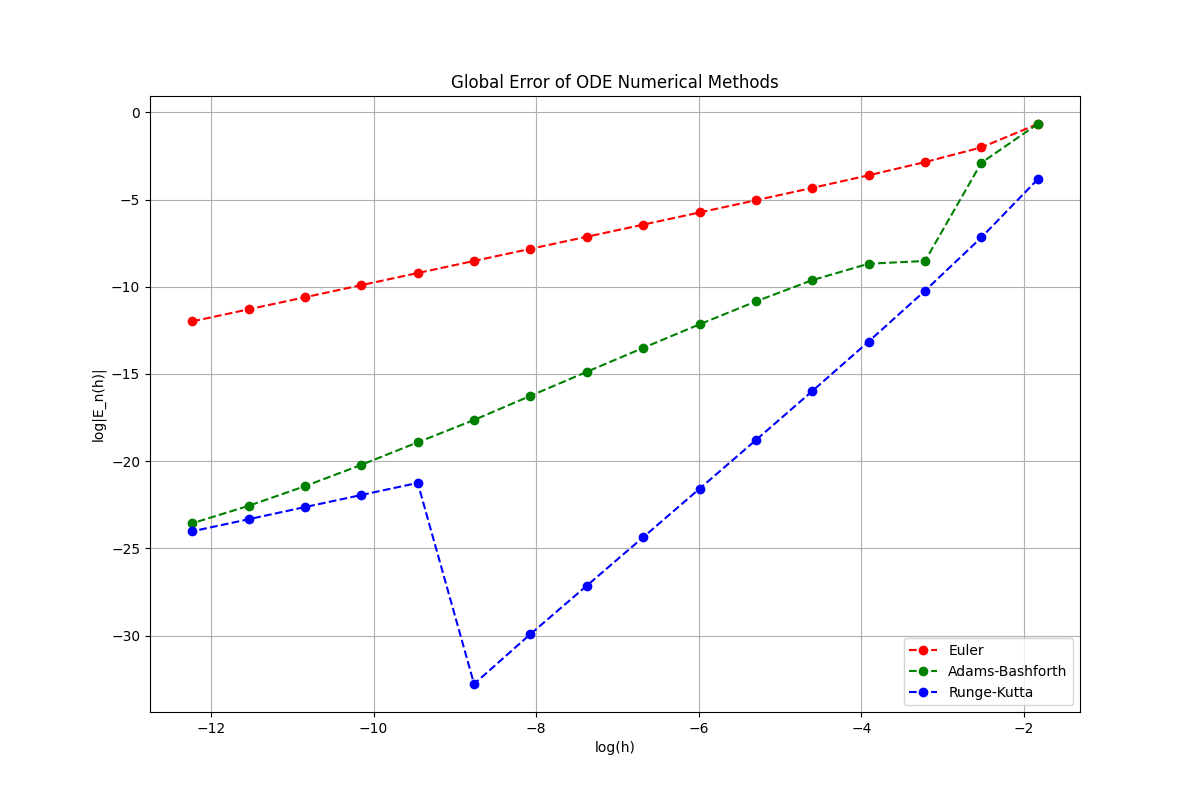
\includegraphics[width=1.0\textwidth]{images/error_comparison.png}
    \caption{Global error asymptotic growth.}
\end{figure}

If the local error is \(O(h^{m+1})\) then the global error should be \(O(h^m)\). We see from the plot that the gradient of the Euler, Adams-Bashforth and Runge-Kutta lines are around \(1\), \(2\) and \(4\) respectively, confirming the accuracies or the orders of the methods. The strange 'kink' for the Runge-Kutta method can be attributed to the precision error of the Python program.

\section{Second-Order ODEs}

Consider the second order ordinary differential equation
\[ \frac{d^2y}{dx^2} + p^2(1+x)^{-\alpha}y = 0, \]
where \(y = y(x)\) is subject to the boundary condition \(y(0) = y(1) = 0\). This equation has an explicit analytic form only for special values of \(\alpha\). For instance, take \(\alpha = 2\). Then,
\[ \frac{d^2y}{dx^2} + \left(\frac{p}{1+x}\right)^2y = 0. \]
Consider the substitution \(e^z = 1+x\), so that by implicit differentiation \(\frac{dz}{dx}e^z = 1\), or \(\frac{dz}{dx} = \frac{1}{e^z} = \frac{1}{1+x}\). By the chain rule,
\[ \frac{dy}{dz} = \frac{dy}{dz} \frac{dz}{dx} = \frac{dy}{dz} \frac{1}{1+x}, \]
and differentiating again
\[ \frac{d^2y}{dx^2} = \frac{d}{dx}\left(\frac{dy}{dz} \frac{1}{1+x}\right) = \frac{1}{(1+x)^2}\left(\frac{d^2y}{dz^2} - \frac{dy}{dz}\right). \]
Substituting into our original ODE and factoring yields
\[ \frac{1}{(1+x)^2}\left(\frac{d^2y}{dz^2} - \frac{dy}{dz} + p^2y\right) = 0. \]
Here, the characteristic equation gives (perhaps) two roots
\[ r_{\pm} = \frac{1 \pm \sqrt{(1-2p)(1+2p)}}{2}. \]
Let \(\omega = \frac{\sqrt{4p^2-1}}{2}\). Substituting for \(z = \log(1+x)\), we have the general solutions
\begin{eqnarray*}
    y = \sqrt{1+x}[A\cos(\omega\log(1+x)) + B\sin(\omega\log(1+x))] & \quad \mbox{when} & \quad p > \frac{1}{2}\\
    y = e^{\frac{z}{2}}(A + Bz) = \sqrt{1+x}[A + B(\log(1+x))] & \quad \mbox{when} & \quad p = \frac{1}{2}\\
    y = Ae^{zr_+} + Be^{z_-} = A(1+x)^{r_+} + B(1+x)^{r_-} & \quad \mbox{when} & \quad p < \frac{1}{2}.
\end{eqnarray*}
Under the initial condition \(y(0) = 0\), and \(y'(0) = 1\),  we obtain
\begin{eqnarray*}
    y = \frac{1}{\omega}\sqrt{1+x}\sin(\omega\log(1+x)) & \quad \mbox{when} & \quad p > \frac{1}{2}\\
    y = \sqrt{1+x}\log(1+x) & \quad \mbox{when} & \quad p = \frac{1}{2}\\
    y = \frac{1}{2\omega}((1+x)^{r_-} - (1+x)^{r_+}) & \quad \mbox{when} & \quad p < \frac{1}{2}.
\end{eqnarray*}

By taking into account the boundary conditions \(y(0) = y(1) = 0\), we see that non-trivial solutions exist only when the roots are complex conjugate. In particular, for two real roots the left boundary condition implies \(A = -B\), whilst the right boundary condition fixes \(r_+ = r_-\) giving a contradiction. For the repeated root, the left boundary condition implies \(A = 0\) and the right boundary condition implies \(B = 0\), which is trivial. To find the eigenvalues and eigenfunctions in the complex conjugate roots case, note that \(y(0) = 0\) gives \(A = 0\), and \(y(1) = 0\) gives \(\sqrt{2}B\sin(\omega\log(2)) = 0\) which is satisfied whenever
\[ \sin(\omega\log(2)) = 0 \Rightarrow \omega\log(2) = n\pi, \]
for any integer \(n\). Solving for \(p\) gives
\[ p^2 = \frac{1}{4} + \left(\frac{n\pi}{\log(2)}\right)^2, \]
with eigenfunctions
\[ y_n(x) = C_n\sqrt{1+x}\sin\left(\frac{n\pi}{\log(2)}\log(1+x)\right). \]
for some normalisation constant \(C\). Taking \(n = 1\) gives the smallest positive eigenvalue with corresponding eigenfunction.

Notice that the initial value problem is equivalent to
\[ \frac{dy}{dx} = f(x, y, z) = z, \quad \frac{dz}{dt} = g(x, y, z) = -p^2(1+x)^{-\alpha}y, \]
which is a two-dimensional system of ODEs where we can find a numerical approximation using any of our numerical methods. We can generalise our Runge-Kutta algorithm to systems of ODEs of any dimension:

\begin{minted}[autogobble, linenos]{python}
    def runge_kutta_2(f, h, x_start, y_start, x_end):
        n = int((x_end - x_start) / h + 1)
        x = np.array([round(x_start + i * h, 8) for i in range(n)])
        y = np.zeros((n, len(y_start)))
        y[0] = y_start
        
        for i in range(n - 1):
            k1 = np.array([f_j(x[i], y[i]) for f_j in f])
            k2 = np.array([f_j(x[i] + h / 2, y[i] + h / 2 * k1) for f_j in f])
            k3 = np.array([f_j(x[i] + h / 2, y[i] + h / 2 * k2) for f_j in f])
            k4 = np.array([f_j(x[i] + h, y[i] + h * k3) for f_j in f])
            y[i + 1] = y[i] + (h / 6) * (k1 + 2*k2 + 2*k3 + k4)
        return x, y
\end{minted}

Let us verify this works by computing for \(\alpha = 2\), \(p = 4\) and \(h = 0.1\) and plotting the graphs of the numerical approximations and the analytic solution,
\[
    y(x) = \frac{2}{\sqrt{63}} \sqrt{1 + x} \sin\left( \frac{\sqrt{63}}{2} \ln(1 + x) \right).
\]
The table of values is as follows:
\begin{verbatim}[Output]
    x       y_n                     y_e
    0.0     0.0 0.0
    0.1     0.09758125472411187     0.09759549816842479
    0.2     0.18272312117106265     0.18274636279550227
    0.3     0.2479186041339051      0.2479444245140176
    0.4     0.28989277184957724     0.2899155469218728
    0.5     0.30836431675958287     0.3083798679961832
    0.6     0.30500244336254995     0.3050080945271249
    0.7     0.2826240098371243      0.2826184042357771
    0.8     0.24461124421413233     0.24459408777074218
    0.9     0.19450975230222955     0.19448155576427475
    1.0     0.13576482860337882     0.13572667829769547
\end{verbatim}

\begin{figure}
    \centering
    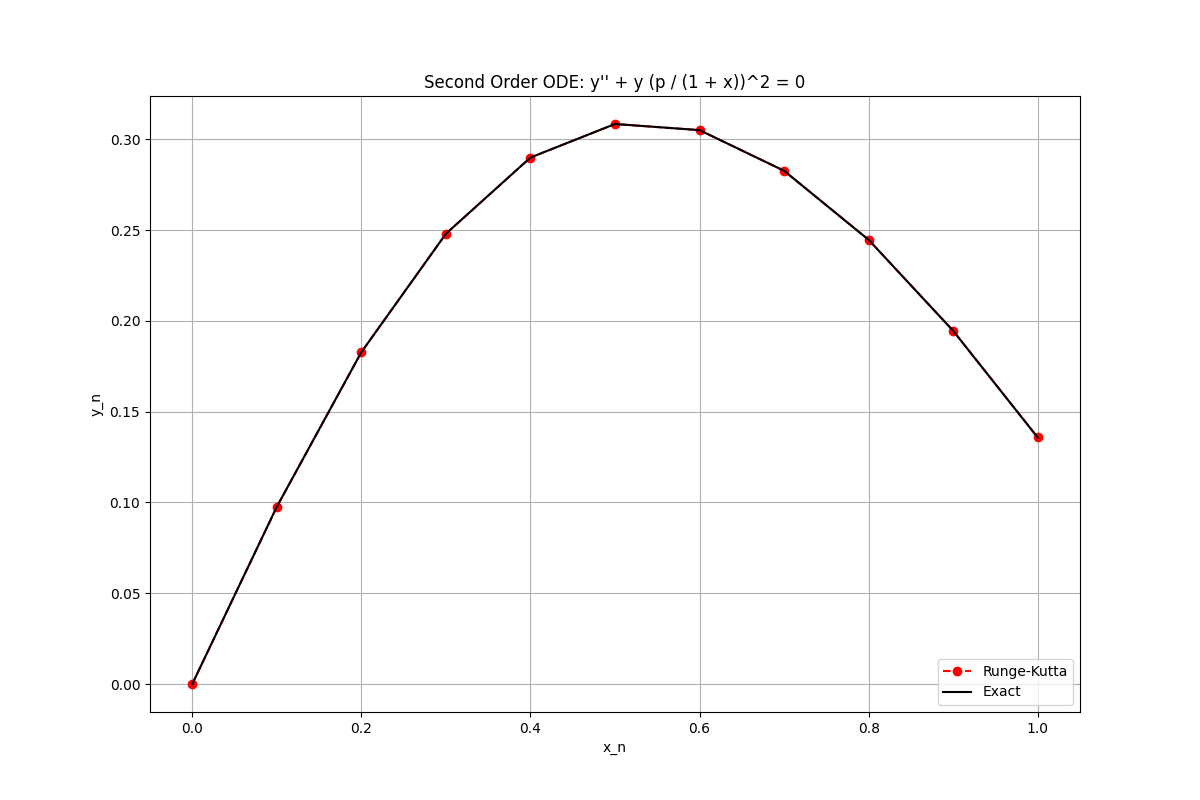
\includegraphics[width=1.0\textwidth]{images/second_order.png}
    \caption{Comparison of the numerical method and analytic solution.}
\end{figure}

Furthermore, by considering the global error at \(x_n = 1\) for step-sizes \(h = 0.1 / 2^k\) for \(k = 0, \dots, 12\):
\begin{verbatim}[Output]
    h               E_n
    0.1             3.815030568335431e-05
    0.05            2.768830547117407e-06
    0.025           1.8294544668062684e-07
    0.0125          1.1707158659168826e-08
    0.00625         7.396478152177366e-10
    0.003125        4.64672744726613e-11
    0.0015625       2.911698659957551e-12
    0.00078125      1.8215984276537256e-13
    0.000390625     1.3112655405933538e-09
    0.0001953125    6.556297726945104e-10
    9.765625e-05    3.2781763414924114e-10
    4.8828125e-05   1.6390788726283745e-10
    2.44140625e-05  8.195441547620419e-11
\end{verbatim}
We see that the magnitude of the global error decreases when the step-size decreases and is relatively small compared to \(Y_n\), which is consistent with our method being accurate and stable. This is also true when setting \(p = 5\) too.

\section{Linear Interpolation Method}

Below is an algorithm that implements linear interpolation. This is similar to the bisection method for a function \(\phi\) on an interval \([a, b]\), except instead of taking the midpoint \(m = \frac{a+b}{2}\) on the domain as the next iteration, we take the linear interpolate by assuming
\[ \phi(a)\frac{b - p}{b -a} + \phi(b)\frac{p -a}{b - a} = 0, \]
which we can solve for \(p\) to obtain
\[ p = \frac{\phi(b)a - \phi(a)b}{\phi(b) - \phi(a)}. \]
We end at the iteration where the value of \(|\phi(p)| < \epsilon\) is less than some specified value.

\begin{minted}[autogobble, linenos]{python}
    def interpolate(func, a, b, err):
        func_a = func(a)
        func_b = func(b)
        if func_a * func_b > 0:
            raise Exception("No root found")
        func_mid = 1
    
        while func_mid != 0:
            mid = (func_b * a - func_a * b) / (func_b - func_a)
            func_mid = func(mid)
            if (abs(func_mid) < err):
                return mid
            if func_a * func_mid < 0:
                b = mid
                func_b = func_mid
            else:
                a = mid
                func_a = func_mid
\end{minted}

Using this, we take \(\phi\) to be the numerical solution \(Y_n\) of the second-order ODE with \(\alpha = 2\) at \(x_n = 1\) for a sufficiently small step-size \(h \). In order to find a good estimate for the smallest positive eigenvalue, we set the error tolerance to be \(\pm 5\cdot 10^{-6}\). We also know that \(\phi(4) > 0\) whilst \(\phi(5) < 0\). In order to ensure our global error is less than the error tolerance but without adding unnecessary computational burden, we shall take \(h = 0.025\) and \(\epsilon < 10^{-7}\).

\begin{verbatim}[Output]
    p                   phi(p)
    4                   0.13572686124314215
    5                   -0.08584314406303951
    4.6125687502493165  -0.011333444038074673
    4.565360133096318   -0.0011957618500541348
    4.560422774583707   -0.0001228919412473231
    4.559915806841232   -1.2595481585379875e-05
    4.559863851356773   -1.2905780998988259e-06
    4.559858527862598   -1.3223344648774504e-07
    4.559857982414558   -1.3548682530062361e-08
\end{verbatim}
Our estimate is very close to the analytic solution of 
\[ p = \sqrt{1/4 + \left(\frac{\pi}{\log(2)}^2\right)}.\]
Indeed, plotting the corresponding eigenfunction gives us a very close approximation to the analytic solution.

\begin{figure}
    \centering
    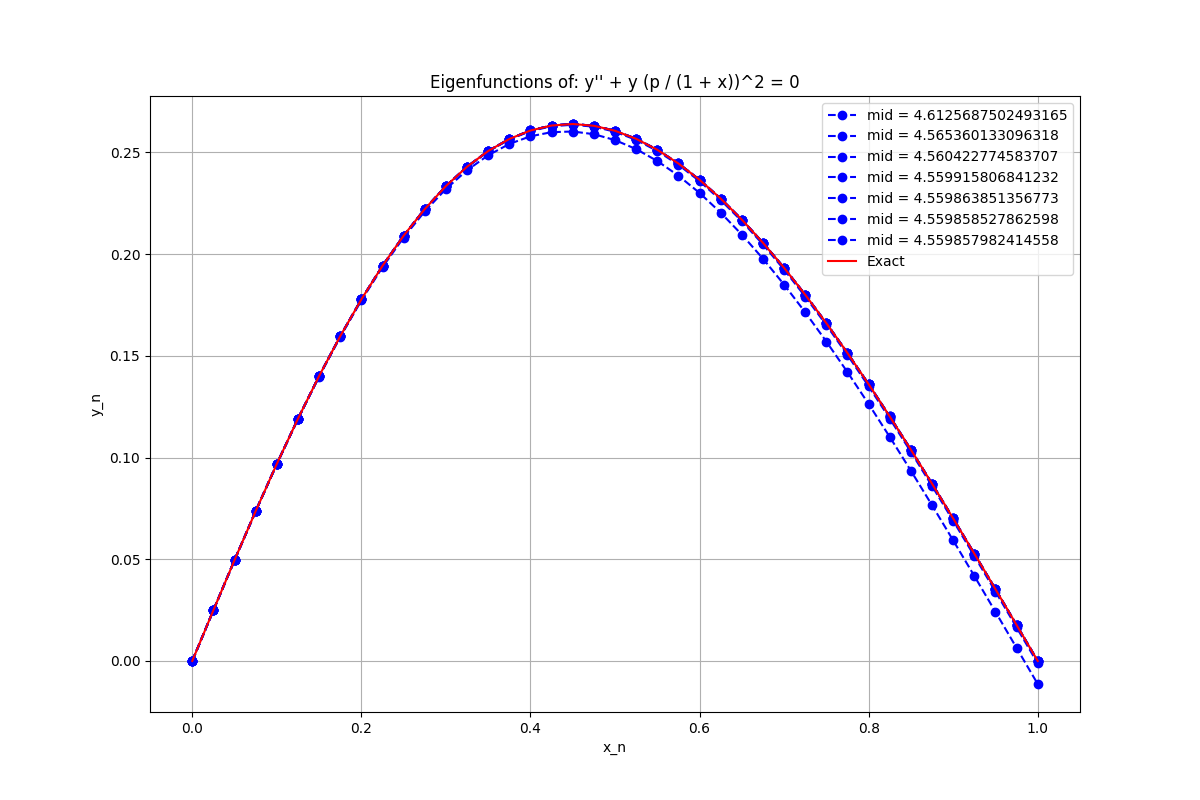
\includegraphics[width=1.0\textwidth]{images/eigenfunction.png}
    \caption{Iterations of the eigenfunction.}
\end{figure}

Now we consider the case where \(\alpha = 10\). This second-order ODE now has no analytic solution. Wentzel–Kramers–Brillouin theory gives us that our Sturm-Liouville boundary value problem has positive eigenvalues \(p^2\) which are asymptotic to
\[ p_n \sim \frac{n \pi}{\int_0^1 \sqrt{\frac{1}{(1+x)^{10}}}\,dx} = \frac{64n\pi}{15}, \]
where this approximation is apparently surprisingly accurate even for small values of \(n\).

Let us take the closest integer value for the boundary for our interpolation algorithm for \(n = 1,2,3,4,5\). This gives \(13, 27, 40, 54, 67\) as a rough approximation for the first five eigenvalues. We shall take the initial boundary guesses to be \(\pm 1\) around these initial guesses. We shall stay with the same choice of \(h = 0.025\) and \(\epsilon < 10^{-7}\) to ensure accuracy up to \(5\cdot 10^{-6}\). Running this through the Runge-Kutta method and interpolating between negative and positive values, this yields the following eigenvalues:

\begin{verbatim}[Output]
    n   p_n
    1   12.576599414621578
    2   26.182926534158952
    3   39.71239684069927
    4   53.20449685039944
    5   66.68010354445472
\end{verbatim}

Taking the intermediate values in Runge-Kutta and normalising using the energy normalisation,
\[ \int_0^1 (1+x)^{-10}[p_n y_n(x)]^2 \,dx = 1, \]
allows us to plot the corresponding eigenfunctions. These resemble oscillations with evolving amplitude which physically manifests from a non-uniformly mass distributed string. The potential \((1+x)^{-10}\) is concentrated near \(x = 0\) and decays rapidly at \(x=1\). The eigenfunctions increase in frequency as \(p_n \to \infty\). This corresponds with \(p\) being proportional to the length of the string, the angular frequency, the square root of density of the string but inversely proportional to the square root of the tension of the string.
\begin{figure}
    \centering
    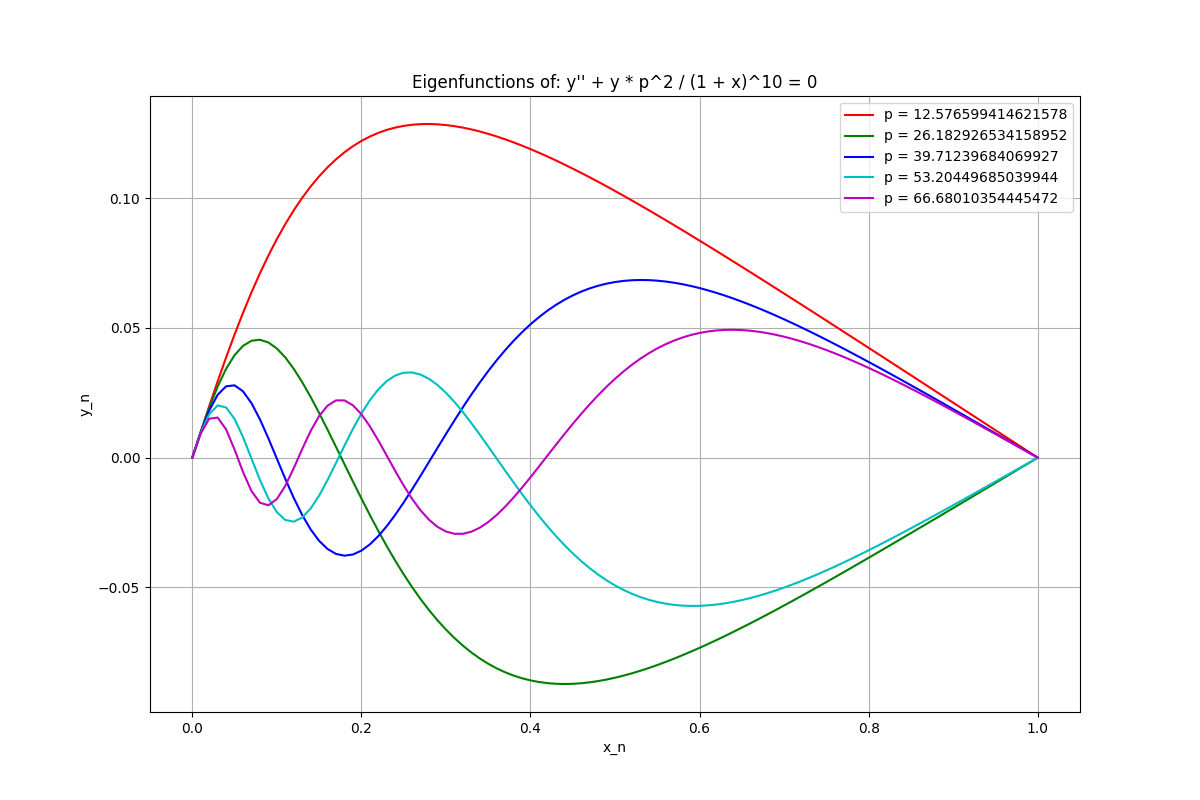
\includegraphics[width=1.0\textwidth]{images/non_analytic_eigenfunction.png}
    \caption{Eigenfunctions for \(\alpha = 10\).}
\end{figure}

\section{Solving ODEs in Python}

In Python, there are several in-built functions for solving initial value problems. A common one is in SciPy, namely the integrate.solve\_ivp function.

\begin{minted}[autogobble, linenos]{python}
    from scipy.integrate import solve_ivp
    import numpy as np
    f = lambda t, y: -8 * y + 6 * math.exp(-2 * t)
    t_eval = np.arange(0, 2, 0.08)
    sol = solve_ivp(f, [0, 2], [0], t_eval = t_eval)
\end{minted}

This gives the following output:

\begin{verbatim}[Output]
 message: The solver successfully reached the 
          end of the integration interval.
 success: True
  status: 0
       t: [ 0.000e+00  8.000e-02 ...  1.840e+00  1.920e+00]
       y: [[ 0.000e+00  3.248e-01 ...  2.522e-02  2.151e-02]]
     sol: None
t_events: None
y_events: None
    nfev: 104
    njev: 0
     nlu: 0
\end{verbatim}

The plot of the approximation is incredibly close to the analytic solution. The plot is not particularly interesting to look at due to the superimposition of the two functions. Instead we plot the difference or error and notice that the magnitude is very small.

\begin{figure}
    \centering
    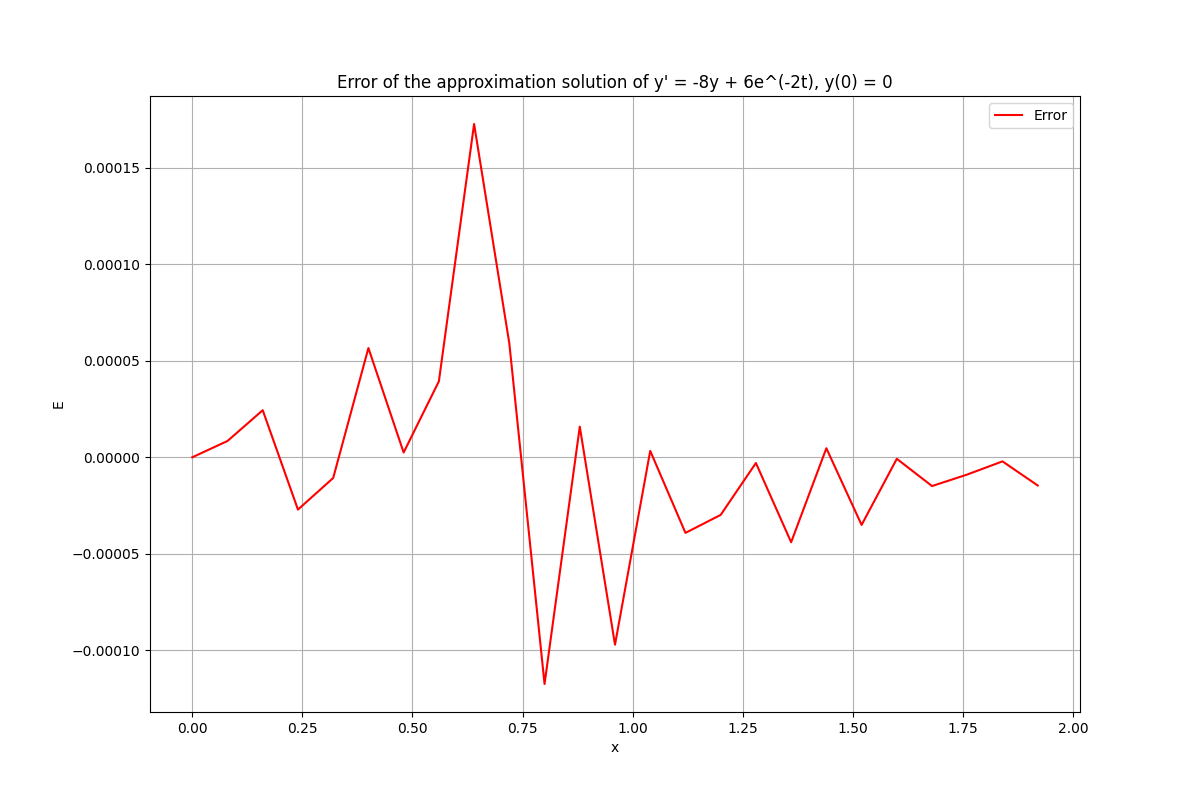
\includegraphics[width=1.0\textwidth]{images/error_python.png}
    \caption{Error between the approximate and analytic solutions is quite small.}
\end{figure}

The solve\_ivp function has a parameter than control the tolerance too. This would be useful in further reducing the magnitude of the error.

\section{Conclusion}

To summarise, there are explicit, implicit, and predictor-corrector methods for numerically solving initial value problems. The accuracy of the scheme used depends on its order of approximation of the ODE. The stability of the scheme used depends on the ODE, the scheme, and the choice of parameters such as step-size. For instance, the explicit Euler method is first-order accurate but not stable whereas the implicit Euler method is stable but not accurate. 

The trapezium method which takes an average of the implicit and explicit Euler methods is both stable and second-order accurate. The Adams-Bashforth two-step method is also both stable and second-order accurate.  Finally, we have also seen that the Runge-Kutta fourth order method is fourth-order accurate and stable.

\end{document}